\documentclass[12pt, a4paper, twoside]{article}
\usepackage{format}
\usepackage{graphicx}

% Do not alter above

% Metadata: put your article information here 
\newcommand{\jtitle}{A Fertility Crisis}
\newcommand{\jauthor}{Justin Lee}
\newcommand{\jaffiliation}{Oakland High School}

% Editors will change these fields after acceptance 
\newcommand{\jvolume}{1}
\newcommand{\jyear}{2025}
% \newcommand{\jdoi}{N/A}  

% References should be placed in refs.bib and cited with \autocite{<source>}
% Quotations can be placed in quote environments: \begin{quote}<your quote>\end{quote}
% Footnotes can be added with \footnote{<your footnote>}

% Your Content

\begin{document}

\maketitle{}

As of 2017, half of the world population resides in a nation with a below replacement level population structure (\cite{frejka2017half}). By 2100, however, 97\% of the world will have a fertility below that of the replacement rate – leaving only six nations able to grow or sustain their population (\cite{thelancet2024dramatic}). Needless to say, declining fertility rates are a hugely existential and complex, if not highly urgent problem. This essay, then, will seek to only briefly investigate the fertility crisis by outlining its causes and repercussions and arguing for what I believe to be the most promising solution. 

Roughly, there are three categories of causes which have led to a fertility crisis: socio-cultural, economic, and biological.  

ocio-cultural factors include secularization, urbanization and an increasing focus on the quality rather than quantity of children. According to a poll by Gallup, people are as non-religious as they have ever been, from 0\% of people identifying as non-religious in 1954 to 21\% in 2022 (\cite{newport2022slowdown}). Then, as religiosity is linked to fertility, this trend has no doubt contributed to a decline in the fertility rate (\cite[p.\ 85]{kearney2023causes}). Urbanization also plays an important role in reducing fertility rates, as when families move into cities, a demand for manual labor, present in the countryside, but  disappears, eliminating a key incentive for parents to have more children (\cite{bricker2021birthrates}). Also, a cultural shift towards having less, rather than more, higher quality has tempered parents’ desire for multiple children (\cite[p.\ 84]{kearney2023causes}).  

Economic factors mainly describe factors general fears regarding the economy, such as fears of job insecurity and the increasing costs of raising children. An excellent example of financial uncertainty causing a decline in fertility is during recessions, as amid such events, fertility rates have consistently fallen (see Figure \ref{fig:1}) (\cite[p.\ 83]{kearney2023causes}). Moreover, when families are burdened by debt or when they have little disposable income, they are less likely to have children (\cite[pp.\ 82, 84]{kearney2023causes}). Exacerbating this problem is the rising costs of raising children; in the last decade alone, the cost of childcare had risen by 28\% (\cite{usafacts2022childcare}). As these trends persist, demand for children will continue to slump (\cites{becker1960economic}{lino2017cost}). 

\begin{figure}[h]
\centering
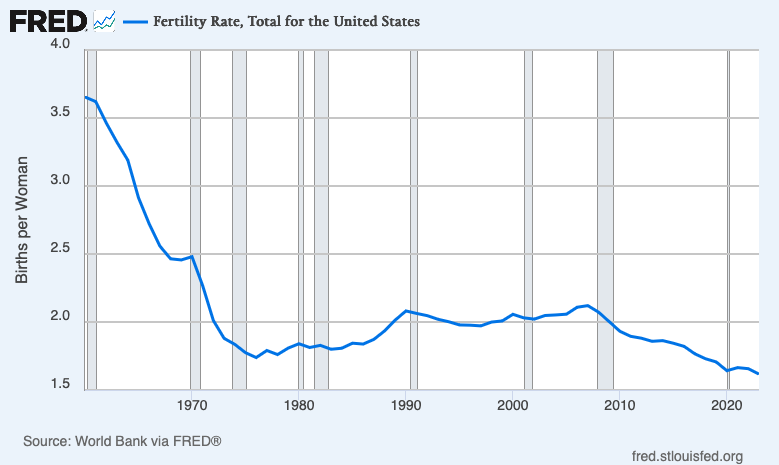
\includegraphics[width=0.9\linewidth]{fredgraph.png}
\caption{US fertility rate trend 1960–2022, overlayed with US recessions. From \emph{Fertility Rate, Total for the United States}, by World Bank, 2024. (\url{https://fred.stlouisfed/series/SPDYNTFRTINUSA}). Copyright 2024 by the Federal Reserve Bank of St.\ Louis.}
\label{fig:1}
\end{figure}

Biological factors relate to the development of contraceptive technology, rising infertility, and reliance on fertility technology such as in vitro fertilization (IVF). In recent decades, contraceptive technologies have increasingly been made available. In fact, from 1955 to 1965, an estimated 40\% of the reduction in fertility rate was facilitated by access to contraception (\cite[p.\ 25]{bailey2010mommas}). Furthermore, studies have shown that biological factors such as poor semen quality, infertility, and increasing rates of testicular cancer caused by environmental pollution have also contributed to a decline in fertility (\cite{skakkebaek2022environmental}).  

Having discussed the causes of the crisis, we can now proceed with discussion of its ramifications. The main consequence of a depressed fertility rate is its macroeconomic effect, as the size of the economy (or GDP) is dependent on the size of its workforce, as well as on the number of pensioners. According to the Solow Growth Model, GDP is directly proportional to workforce size; therefore, if the size of the workforce were to be reduced, then the economy would similarly contract (\cite{solow1956contribution}). Although ceteris paribus, per capita GDP would remain constant while the workforce shrinks, a diminished GDP means that overall spending on public goods may decrease, resulting in a tighter defense or education budget (\cite[p.\ 88]{kearney2023causes}). Aside from this, the dependency ratio is also a key factor affected by falling fertility rates. With less working age population and more pensioners, the government must spend more in terms of social benefits and/or the children of the elderly must have greater support for their parents financially, both of which puts strain on the economy (\cite[pp.\ 91–92]{kearney2023causes}). Lastly, inflationary pressure and curtailed innovation have also been proposed as consequences of the fertility crisis (\cites{jones2022end}[p.\ 18{kohler2006low}]).

Despite these detractions, however, there are perks to low fertility. Under such circumstances, the cost of equipping new workers would fall, environmental pressures would ease, and the impact of an increasing skewed dependency ratio is projected to be counterbalanced by increased investment in human capital, hence improving the efficiency of workers (\cites[p.\ 3]{jarzebski2021ageing}{lee2010fertility}[p.\ 7]{lee2014low}). An additional consideration lies in the increasing automation of many industries, such that demand for human labor may decrease in the future. However, in spite of presently addressed concerns, a normative argument could still be made, as by attempting to raise fertility rate, there are only minor drawbacks, while the potential for catastrophic consequences if fertility is left unchecked are immense. 

When considering potential remedies to the fertility crisis, perhaps the most conspicuous solution is pro-natal governmental suasion. Such examples include financial incentives, expanded employment benefits, subsidized childcare, and housing subsidies. Propagandizing efforts to change social perceptions of children may also be adopted through art (see Figure \ref{fig:2}), slogans, and other media (\cite[p.\ 37]{kohler2006low}). Indeed, this is the method adopted by many nations around the world today.

\begin{figure}
\centering

\includegraphics[width=\linewidth]{top-600.jpg}
\caption{A sculpture in Wuhan, a city in central China, depicted a joyful family of three. Recently, two more children were added. From \emph{Three Is Best: How China’s Family Planning Propaganda Has Changed}, by Isabelle Qian and Pablo Robles, 2024. (\url{https://www.nytimes.com/interactive/2024/03/09/world/asia/china-childbirth-propaganda.html}). Copyright 2024 by The New York Times Company}
\label{fig:2}
\end{figure}

For an example, we can turn to Singapore, which began to introduce explicitly pro-natal policies beginning in 2001. Singapore initiated policies to make working environments more accessible for those wishing to start a family, subsidized reproductive technologies like IVFs and contraception, and offered low-cost, high-quality formal childcare. These comprehensive measures, however, achieved only limited success, failing to produce long-term, concrete results (\cite{tan2020lessons}).

Rather than direct governmental interference, I argue that the most effective method of combating low fertility rate around the world is through the continued focus on implementation of policies which strengthen and stabilize the overall economy, while adopting a “homeostatic” stance towards population. Through focusing on fundamental issues such as reducing unemployment, promoting free international trade, fostering innovation and other such matters, we absolve people’s insecurities regarding their and their potential children’s future. This mitigates a central motivation in the reduction of fertility, while avoiding superfluous governmental interference. Compared to the interventionist approach, where there exists only a weak correlation between implemented policies and increases in fertility, focusing on improving future economic outlook has historically been an effective promoter of economic stability (\cites[pp.\ 93–97]{kearney2023causes}{stern2022ways}). Additionally, the Easterlin hypothesis states that as labor supply falls and demand rises, wages also grow, generating demand for children and inducing a rebound in fertility (\cites{easterlin1987birth}[p.\ 31]{kohler2006low}). Though such a stance towards population planning is currently theoretical, it seems the most cost-effective and laissez faire solution to the fertility crisis, letting population dynamics simply be influenced by organic economic forces. 

\printbibliography

\end{document}
